% This is samplepaper.tex, a sample chapter demonstrating the
% LLNCS macro package for Springer Computer Science proceedings;
% Version 2.20 of 2017/10/04
%
\documentclass[runningheads]{llncs}
%
\usepackage{graphicx}
\graphicspath{{./images/}}
% Used for displaying a sample figure. If possible, figure files should
% be included in EPS format.
%
% If you use the hyperref package, please uncomment the following line
% to display URLs in blue roman font according to Springer's eBook style:
% \renewcommand\UrlFont{\color{blue}\rmfamily}

\begin{document}
%
\title{LightBulbs - Constraint Logic Programming}
%
%\titlerunning{Abbreviated paper title}
% If the paper title is too long for the running head, you can set
% an abbreviated paper title here
%
\author{Ivo Saavedra - up201707093\and
João Cardoso - up201806531 \\
\small{FEUP-PLOG, 3MIEIC01, Grupo LightBulb}}

%
\authorrunning{F. Author et al.}
% First names are abbreviated in the running head.
% If there are more than two authors, 'et al.' is used.
%
\institute{Faculdade de Engenharia da Universidade do Porto, Rua Roberto Frias, 4200-465 Porto, Portugal}
%
\maketitle              % typeset the header of the contribution
%
\begin{abstract}
This article contains the implementation details of the application developed for the second assignment for the
Logical Programming subject. The goal of this project was to develop a program capable of creating and solving every instance of the Light bulb puzzle. The goal of this puzzle is to find every lit light bulb, considering that a light bulb is only lit if and only if the number inside it is equal to the number of lit neighboring lamps (including itself).

\keywords{PROLOG  \and SICStus \and Lightbulbs.}
\end{abstract}
%
%
%
\section{Introduction}
This article was developed as complement for the second partical assignment of the Logical Programming subject of the 3rd year of the MIEIC course. The goal of this project was to develop an application capable of creating and solving "Lightbulb" type puzzles using the SISCstus prolog development system along with the restriction tools provided by the CLPFD library. The objective of these puzzles is to determine which light bulbs inside a n*n square are turned on. A light bulb is only on when the number of adjacent bulbs (including itself) equals the number attributed to it. This document is organized in the following manner:
	\begin{itemize}
		\item[•] \textbf{Problem Description:} detailed description of the problem being analyzed
		\item[•] \textbf{Approach:} section describing the implementation of the application
		\begin{itemize}
			\item[-] \textbf{Decision Variables:} description of the decision variables and their domains
			\item[-] \textbf{Constraints:} details of the rigid and flexible constraints
		\end{itemize}
		\item[•] \textbf{Solution Presentation:} description of the adopted solution presentation
		\item[•] \textbf{Experiments and Results:}
		\begin{itemize}
			\item[-] \textbf{Dimension Analysis:} results obtained after testing boards of different sizes
			\item[-] \textbf{Search Strategies:} result comparison of different heuristics search functions
		\end{itemize}
		\item[•] \textbf{Conclusions}
		\item[•] \textbf{References}
	\end{itemize}

\section{Problem description}
The Lightbulb puzzle consists of a two dimensonal board consisting of n[1*] light bulbs per line and m[1*] light bulbs per column, where each lightbulb has a number on it.
Each lightbulb is on if and only if it's number is equal to the number of lit neighboring (directly or diagonally adjacent) lightbulbs, including itself. When given a board we must determine all it's possible solutions; the number of solutions may range from one to many, however there are cases in which the board is impossible to solve. Having that in consideration we classified the LightBulbs puzzle as a decision problem.

\section{Approach}

\subsection{Decision Variables}
For this puzzle the decision variables are the values inside each cell of the input board. As previously stated, each board cell as a value representing the number of adjacent bulbs that need to be lit in order for the current cell to be as well.
Taking into consideration that every cell can at most have eight adjacent cells and that for the bulb to be lit we need to have N adjacent lit bulbs plus the current one we come to the conclusion that the maximum number inside a light bulb is 8+1=9. As for the minimum value we came to the conclusion that it should be 1. If the value inside a bulb was equal to zero, then that bulb would always be turned off, because of the constraints of this puzzle.

\subsection{Constraints}
\subsubsection{Elements} \hfill \break
Our problem is a constraint satisfaction problem, therefore, every constraint is a hard constraint, which always have to be true (if they are called).
We have a "results list", where each element is a variable that can be 1, if the corresponding lightbulb is turned off or, otherwise, 0. This list is a flattened version of the list that is returned at the end. It's first element is at line 1 column 1, the second is at line 2 column 1, etc...
[Note: we use nth1, so the first element will be index 1.]

\subsubsection{Element searching} \hfill \break
As previously mentioned, a bulb is only lit when the number inside it is equal to the number of adjacent light bulbs (including itself) that are lit. In order to accomplish this we iterated over all of the input board's cells and for each cell we fetched every adjacent variable. The maximum number of adjacent cells is eight, so for each light bulb we needed eight variables. If the current cell had less than eight neighbors, for instance, if it was in a corner, then the adjacent variables that were out of bounds would take the value of zero.
After having gotten all the adjacent variables we started applying the constraints. The first one being that the sum of all the adjacent variables should be different from the number inside the current bulb.
For example, being given a 4x3 board:
We are using a flattened list, therefore, the line length is 4 and the existing elements are 1 through 16.
The program starts by checking for the first (1 - top left) cell, it first checks for the cell above and to the left of it first (1 - 4 - 1 = -4). Since that element isn't in the board, the would be element's value is zero.
The same thing happens for the element above, above (1 - 4 = -3), above to the right (1 - 4 + 1 = -2) and center to the left (1 - 1 = 0), and, later on, to the element under and to the left.
There isn't a check for itself, since, if an element exists, then it exists.
The other elements are assigned to the corresponding variables (2nd, 5th and 6th elements of the "results list").

Since we repeat the steps above for each list element, when it gets to the end, every element will check wether each adjacent lightbulb (including itself) are lit up.

\subsubsection*{Sum condition} \hfill \break
If the sum of every element in the "results list" is 0, then the "results list" is automatically invalid.

\begin{figure}
	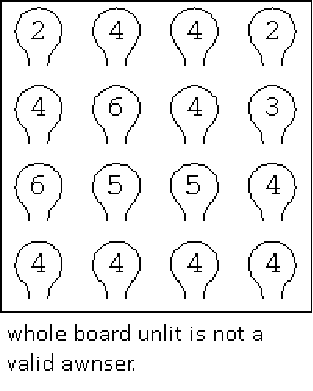
\includegraphics[scale=0.5]{lightbulb_no_whole_board_unlit_restriction}
	\centering
	\caption{No whole board unlit example}
	\centering
	\end{figure}
\clearpage
\subsubsection*{Lockout condition} \hfill \break
First we check if the sum of the neighboring elements, excluding itself, is equal to the number on the lightbulb. If it is, then the current "results list" is automatically invalid.
\begin{figure}
	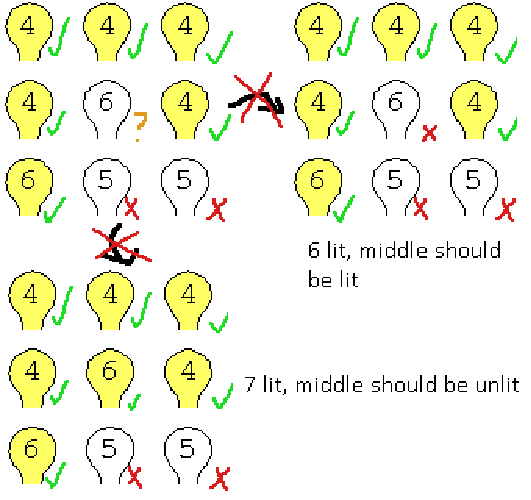
\includegraphics[scale=0.5]{lightbulb_impossible_state}
	\centering
	\caption{Lockout condition example}
	\centering
\end{figure}


\subsubsection*{Light condition} \hfill \break
For each element, we get the sum of the the neighboring elements, excluding itself, plus one (the +1 is because we are assuming that the lightbulb itself is on for this case).
If that sum is equal to the number on the lightbulb we're checking, then the lightbulb can be on, but doesn't necessarily have to be.

\begin{figure}
	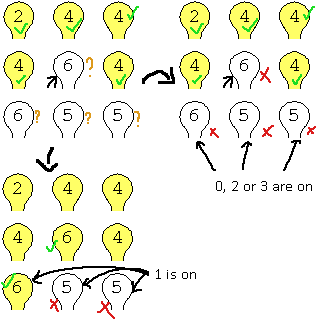
\includegraphics[scale=0.5]{lightbulb_light_condition_example}
	\centering
	\caption{Light condition example}
	\centering
\end{figure}

Each lighbulb lightbulb can always be off, unless it meets the "sum condition" or the "lockout condition".

These restrictions are used both to obtain the solution and to create the problem using a solution.



\clearpage
\section{Solution Presentation}
In order to make the solution more intelligible, the input board is displayed along with the result board, in which the latter
only contains the cells that have a lit bulb, allowing for an easier understanding of the solution. The elapsed time is also displayed for the experiments and results section.
The predicates responsible for displaying the results are called after the solution is obtained. As each board can originate more than one result the solution consists of a list of matrices, each one representing the possible output boards for the original board. The \textbf{showResults} predicate is responsible for iterating over the result matrices and displaying each one in the console.

\begin{figure}[h]
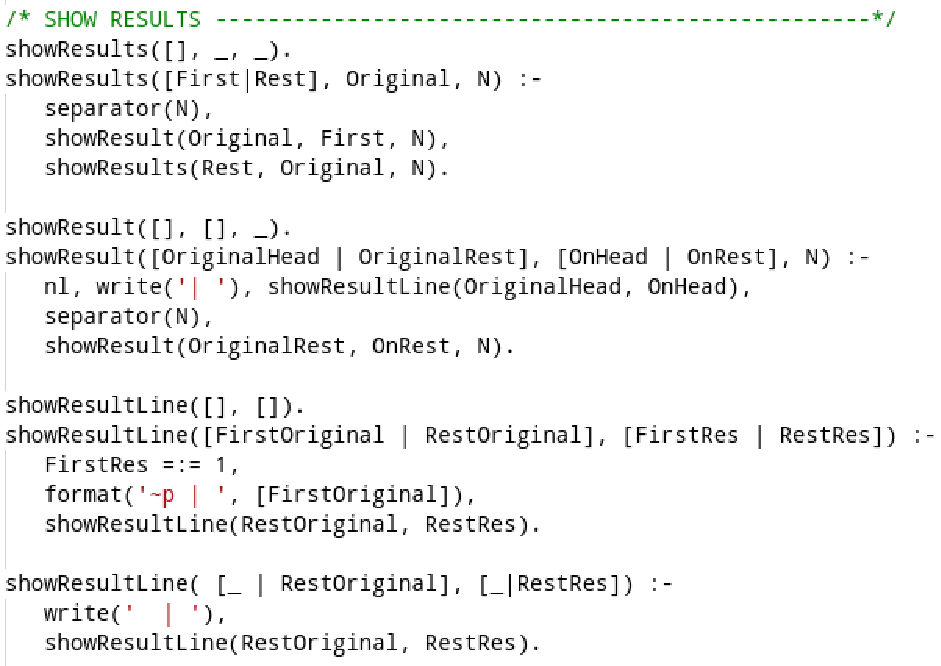
\includegraphics[scale=0.5]{showResults}
\centering
\caption{display result predicates}
\centering
\vspace{5mm}	
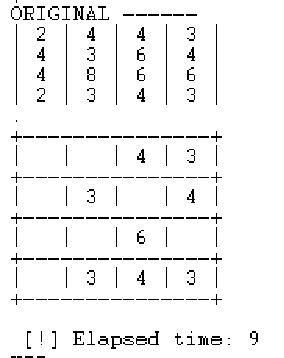
\includegraphics[scale=1]{solutionDisplay}
\centering
\caption{solution display example}
\centering
\end{figure}

\section{Experiments and Results}
\subsection{Dimension Analysis}
The Dimension Analysis graph indicates how our program scales with board size. Board size indicates the length and width of the square board.
Time indicates the time it takes to solve it.
We used a randomly created board with at least one solution.
As expected, the time to solve increased with the board size, however, the spike from 7 to 8 was unexpected. Despite that, the time increase relative to the board size increase seemed to stabilize after that, so we'll assume the spike was an anomaly.
We did one test por board size.

\begin{figure}
	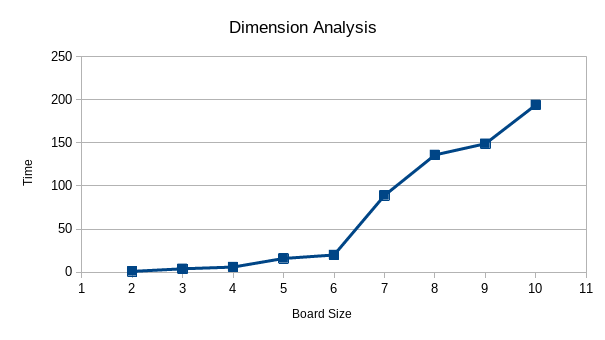
\includegraphics[scale=0.5]{graph}
	\centering
	\caption{Effect of the board size on execution time}
	\centering
\end{figure}

\subsection{Search Strategies}
We ran every our application with different search options but obtained similar results to the ones displayed on figure. 6. These options didn't have that much of an effect on our tests because most off them affect the domain of the variables which in our case was between 0 and 1. Another reason for this, was the fact that this puzzle represents a "satisfaction" problem in which we, for every board, calculate all the possible solutions, therefore the order in which they originated didn't affect the execution time.

\section{Conclusions}
The objective of this project was to develop an application capable of creating and solving light bulb puzzles. At the end of this assignment we feel that our knowledge on the CLPFD prolog module has definitely increased as well as our experience with constraint logical programming.

We also found that the time it took for a board to be solved tended to increase the more solutions there were.

% ---- Bibliography ----
%
% BibTeX users should specify bibliography style 'splncs04'.
% References will then be sorted and formatted in the correct style.
%
% \bibliographystyle{splncs04}
% \bibliography{mybibliography}
%
\begin{thebibliography}{8}
\bibitem{ref_url1}
SICstus Documentation, \url{https://sicstus.sics.se/sicstus/docs/latest4/html/sicstus.html}. Last accessed 4
Jan 2020
\bibitem{ref_url1}
SWI Prolog Documentation, \url{https://www.swi-prolog.org/}. Last accessed 4
Jan 2020
\end{thebibliography}
\end{document}
